\documentclass[
    hyperref={colorlinks,citecolor=DeepPink4,linkcolor=DarkRed,urlcolor=DarkBlue}
]{beamer_class}
\usepackage{soul} % In text mode, the \underline command will enclose its argument in a horizontal box, which doesn't allow linebreaks. Use the \ul command of the soul package instead.
\usepackage[absolute,overlay]{textpos} % insert absolute text positioning with textblock environment
\input{default_preamble.tex}
\input{default_glossary_entries.tex}

%%%%%%%%% beamer configuration %%%%%%%%%
\setlength{\TPHorizModule}{1cm}
\setbeamertemplate{footline}[frame number]
\setbeamertemplate{theorems}[numbered]
\usefonttheme{professionalfonts} % prevent beamer from clashing with some font packages, e.g., bm. See https://tex.stackexchange.com/questions/344162/latex-error-too-many-symbol-fonts-declared-error
\beamertemplatenavigationsymbolsempty
% Theme changed from `seagull` to a cleaner `Madrid` theme with a different color/inner style
\usetheme{Madrid}
\usecolortheme{dolphin}
\useinnertheme{rounded}
\setbeamercovered{transparent} % make \cover overlay transparent but not invisible
\usefonttheme[onlymath]{serif}
\definecolor{alertcolor}{rgb}{.0, .48, .74}
\setbeamercolor{alerted text}{fg=alertcolor}



\title{Geometry-Aided Kalman-Based Tracking Loops for Ionospheric Scintillation Monitoring}
\author{Rubem Vasconcelos Pacelli}
\institute[ITA \& UFC]{Instituto Tecnológico de Aeronáutica (ITA) \& Universidade Federal de Ceará (UFC)}
\date{\today}

\setbeamertemplate{title page}{%
	\vbox{}%
	\vfill
	\begin{center}
		{\usebeamerfont{title}\usebeamercolor[fg]{title}\inserttitle\par}
		\vspace{1.5em}
		{\usebeamerfont{author}\insertauthor\par}
		\vspace{0.75em}
		{\usebeamerfont{institute}\insertinstitute\par}
		\vspace{1.0em}
		{\usebeamerfont{date}\insertdate\par}
	\end{center}
	\vfill
}
 
\begin{document}
 
\frame[noframenumbering,plain]{\titlepage}
 
\begin{frame}
	\frametitle{Outline}
	\tableofcontents[pausesections]
\end{frame}

\section{Introduction}
\begin{frame}[<+->][t]{Ionospheric Scintillation}%[<+->][t]{Ionospheric Scintillation}
    \begin{columns}
		\column{0.5\textwidth}
        \begin{visibleenv}<.->
        \begin{figure}[t]
            \centering
            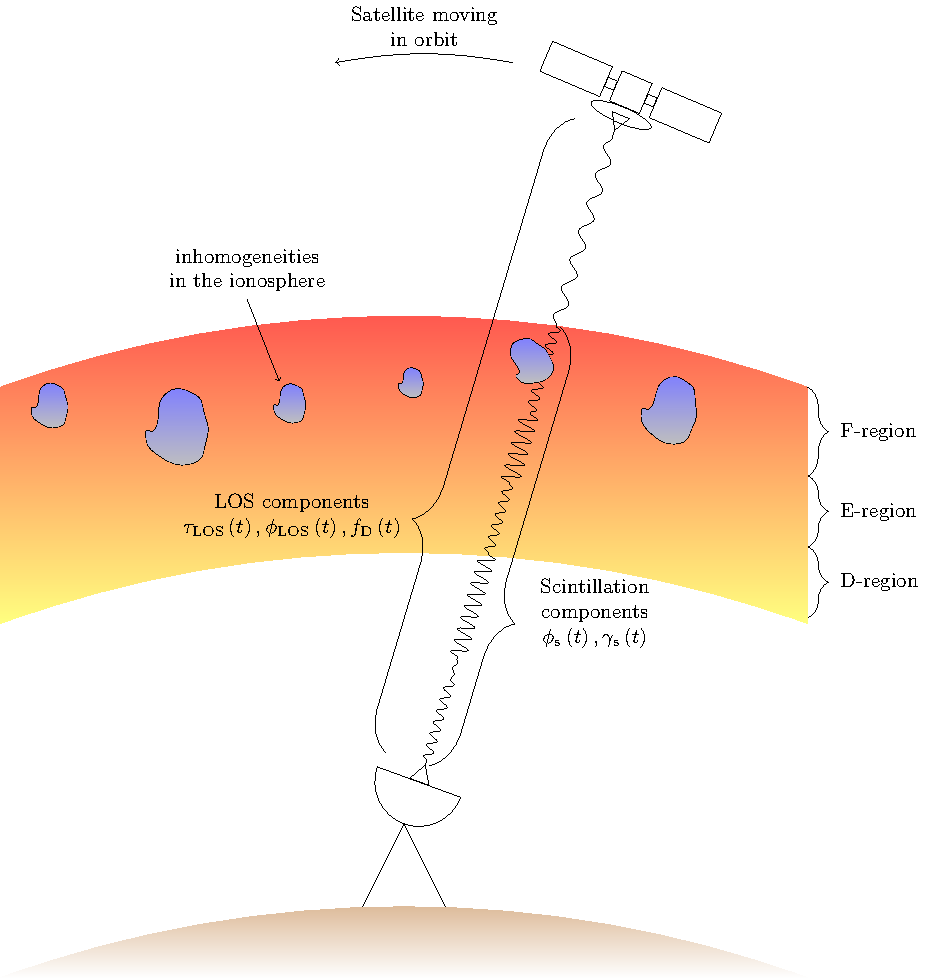
\includegraphics[scale=0.38]{figs/ionospheric_scint/main.pdf}
            \caption{Ionospheric scintillation -- an overview.}
        \end{figure}
        \end{visibleenv}
		\column{0.5\textwidth}
        \begin{visibleenv}<+->
		\begin{figure}[t]
			\centering
			\begin{tabular}{@{}c@{\hspace{0.35em}}c@{}}
				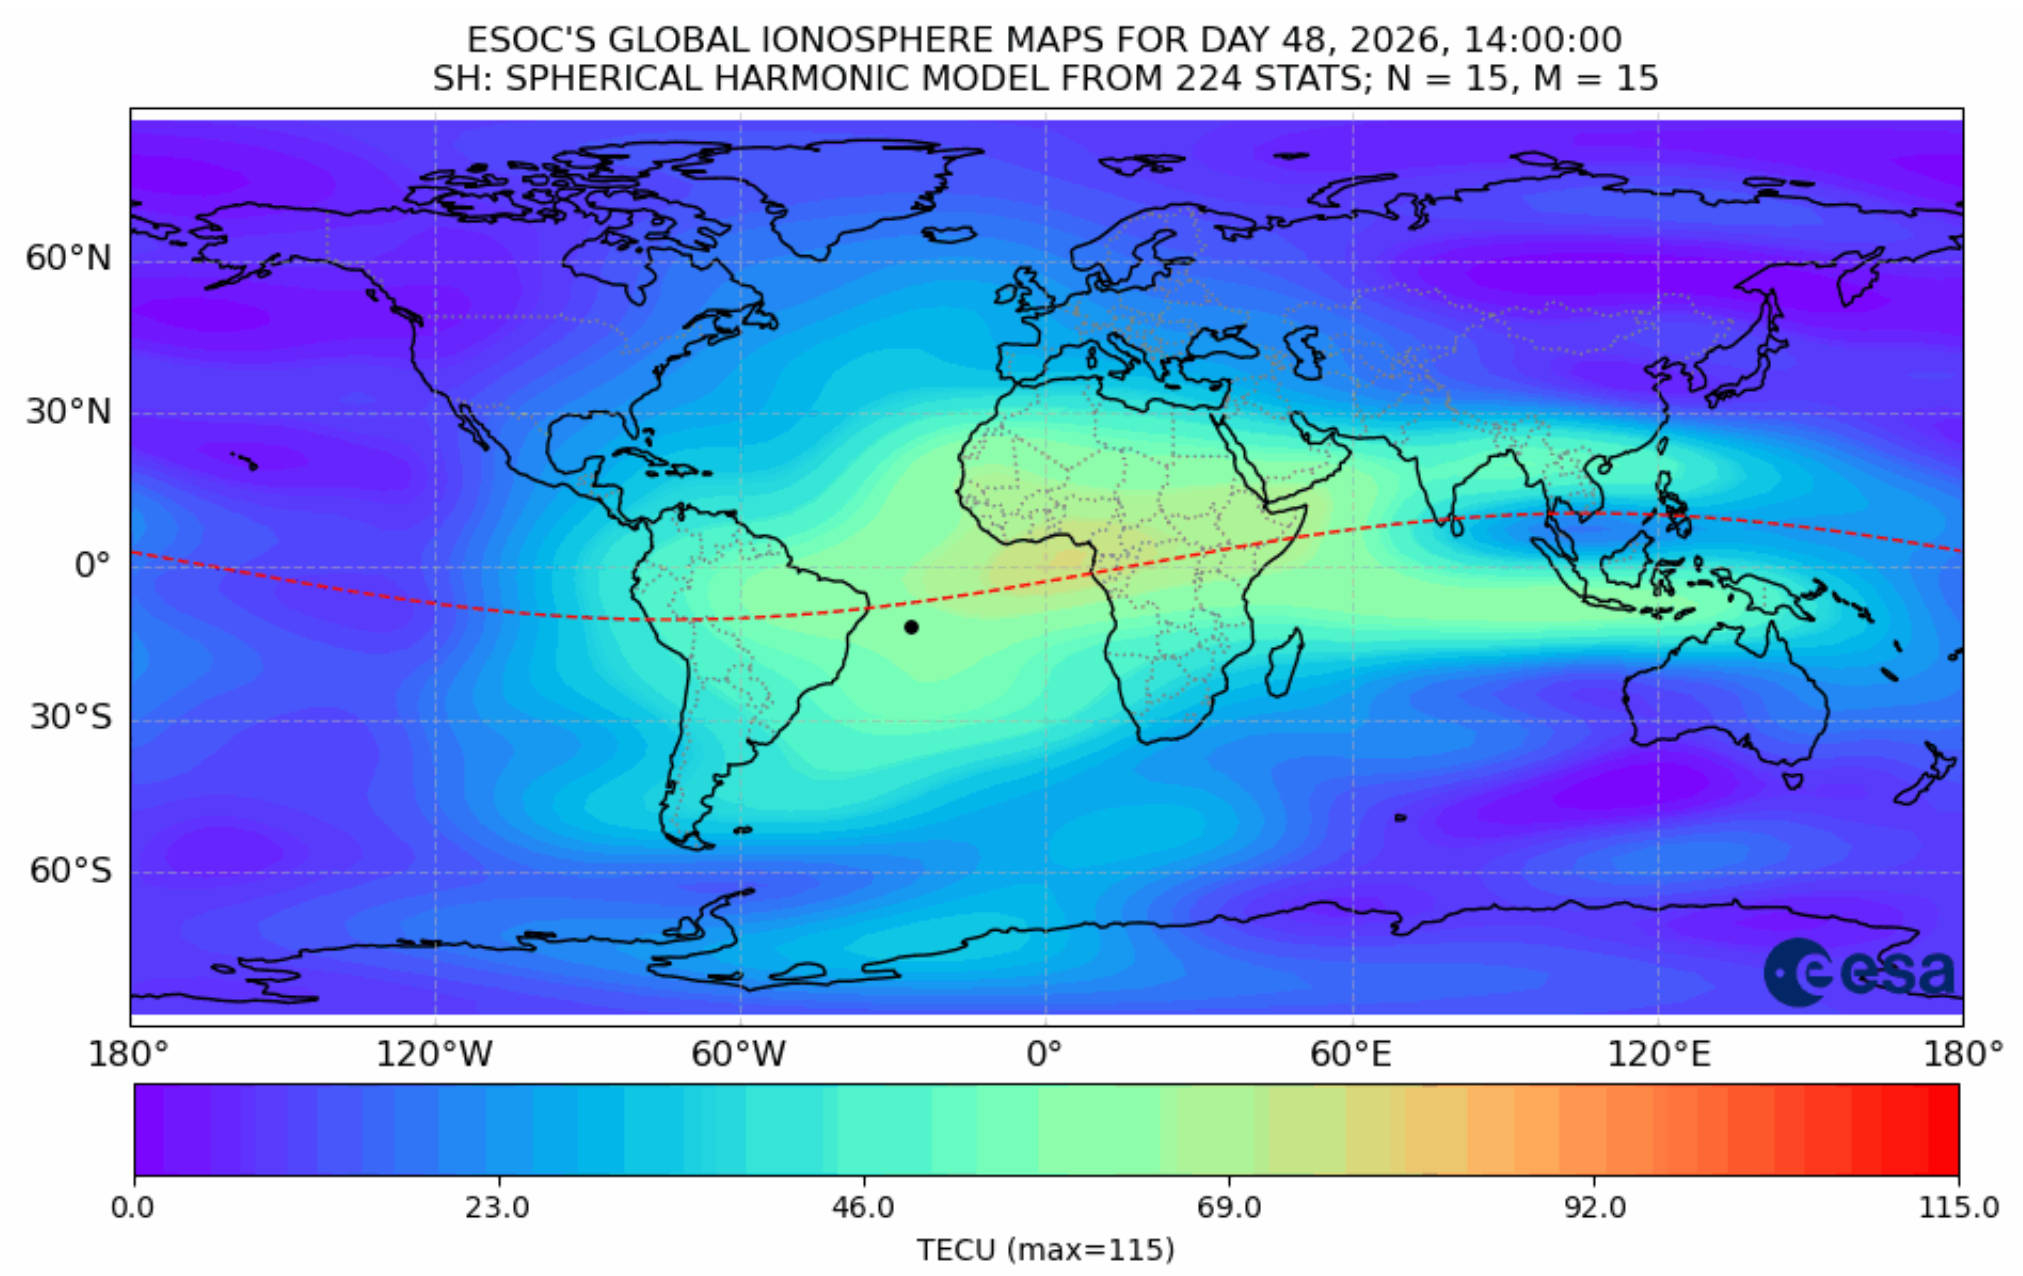
\includegraphics[width=0.47\linewidth]{figs/TECU_2pm.png} &
				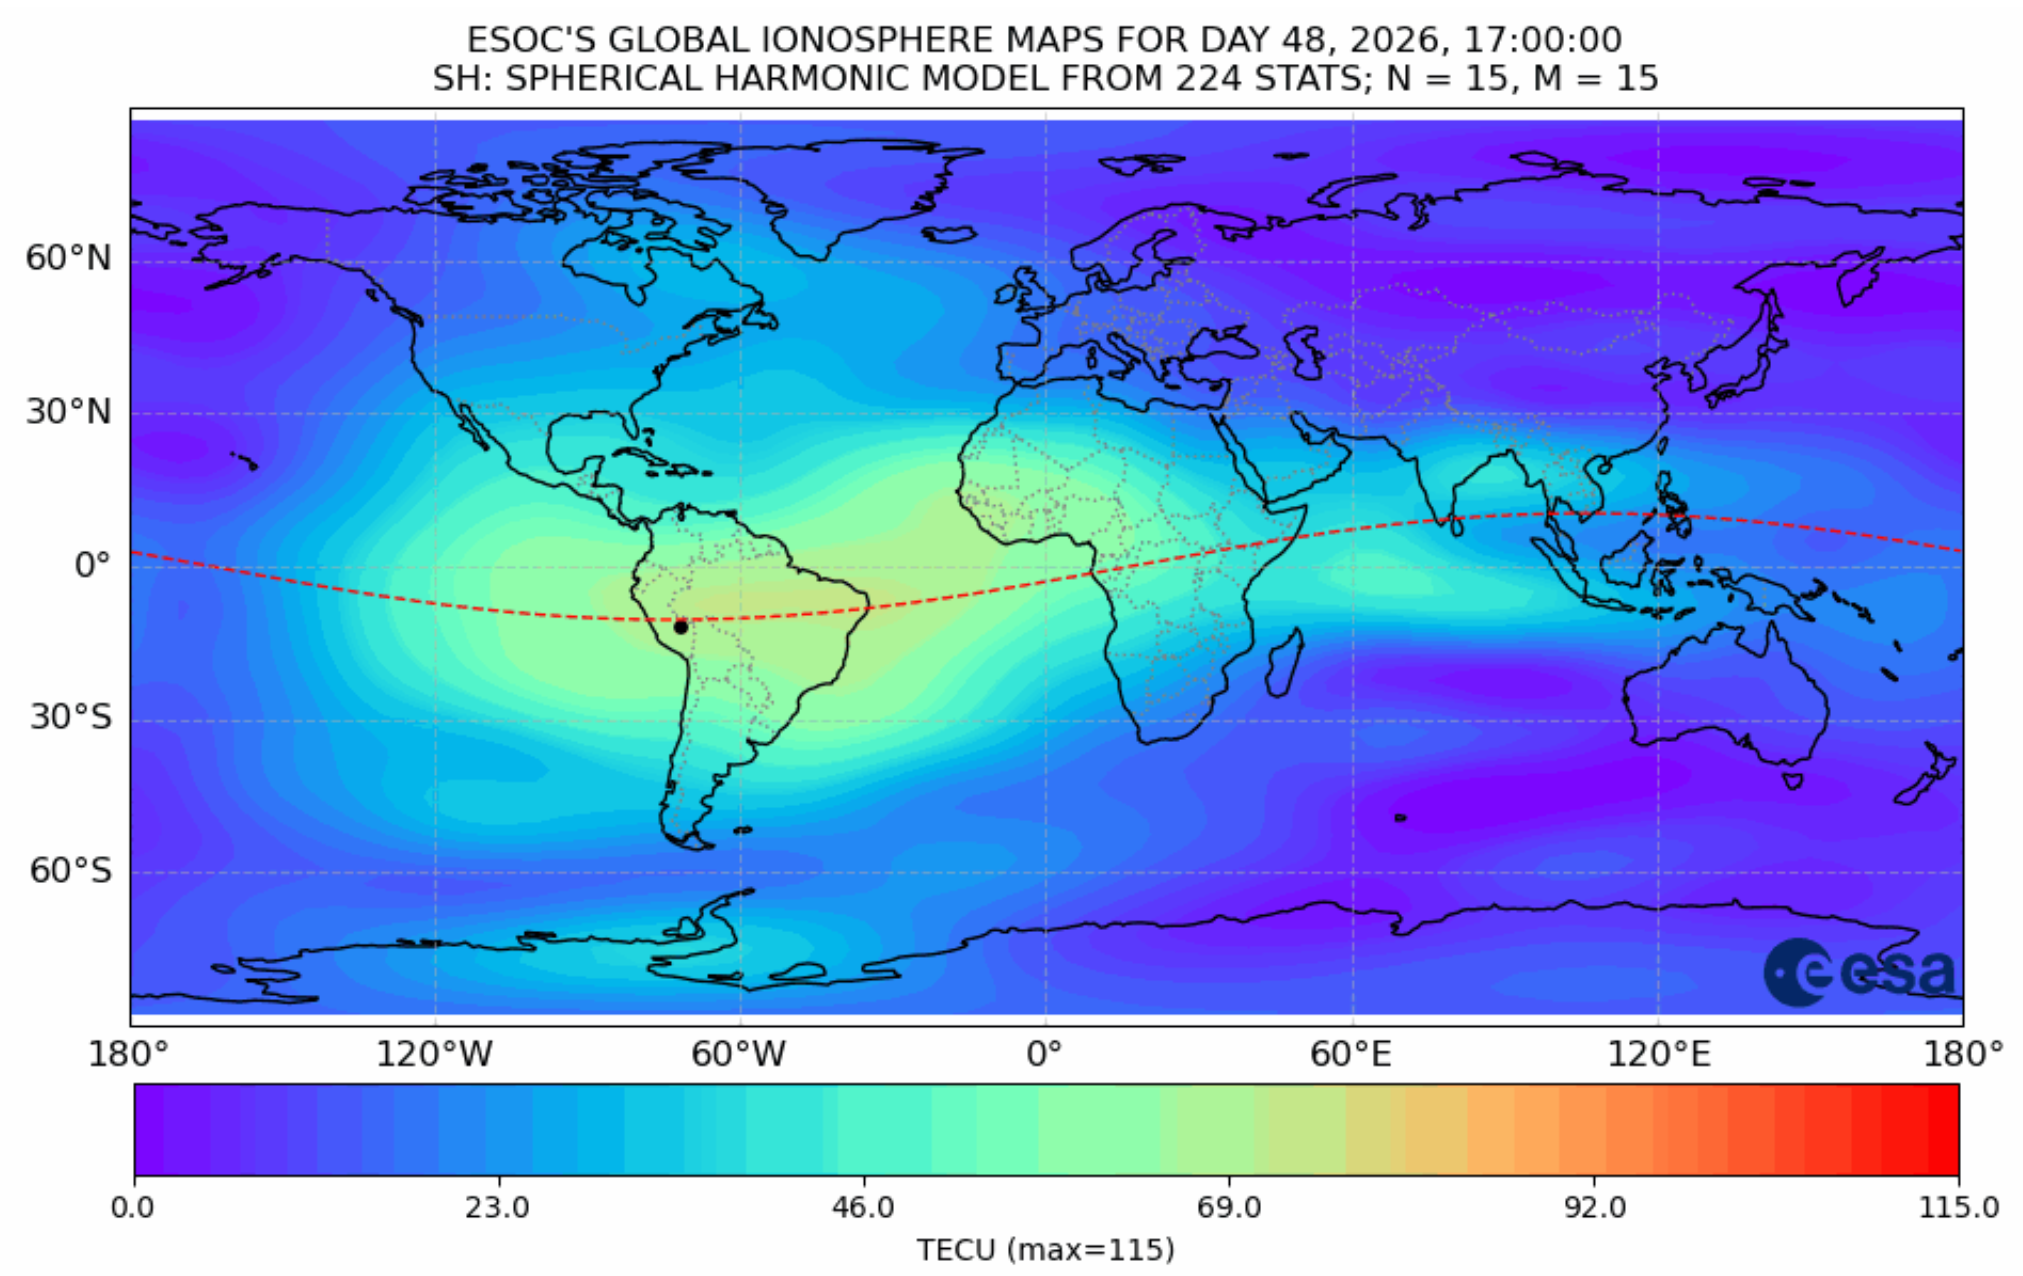
\includegraphics[width=0.47\linewidth]{figs/TECU_5pm.png} \\
				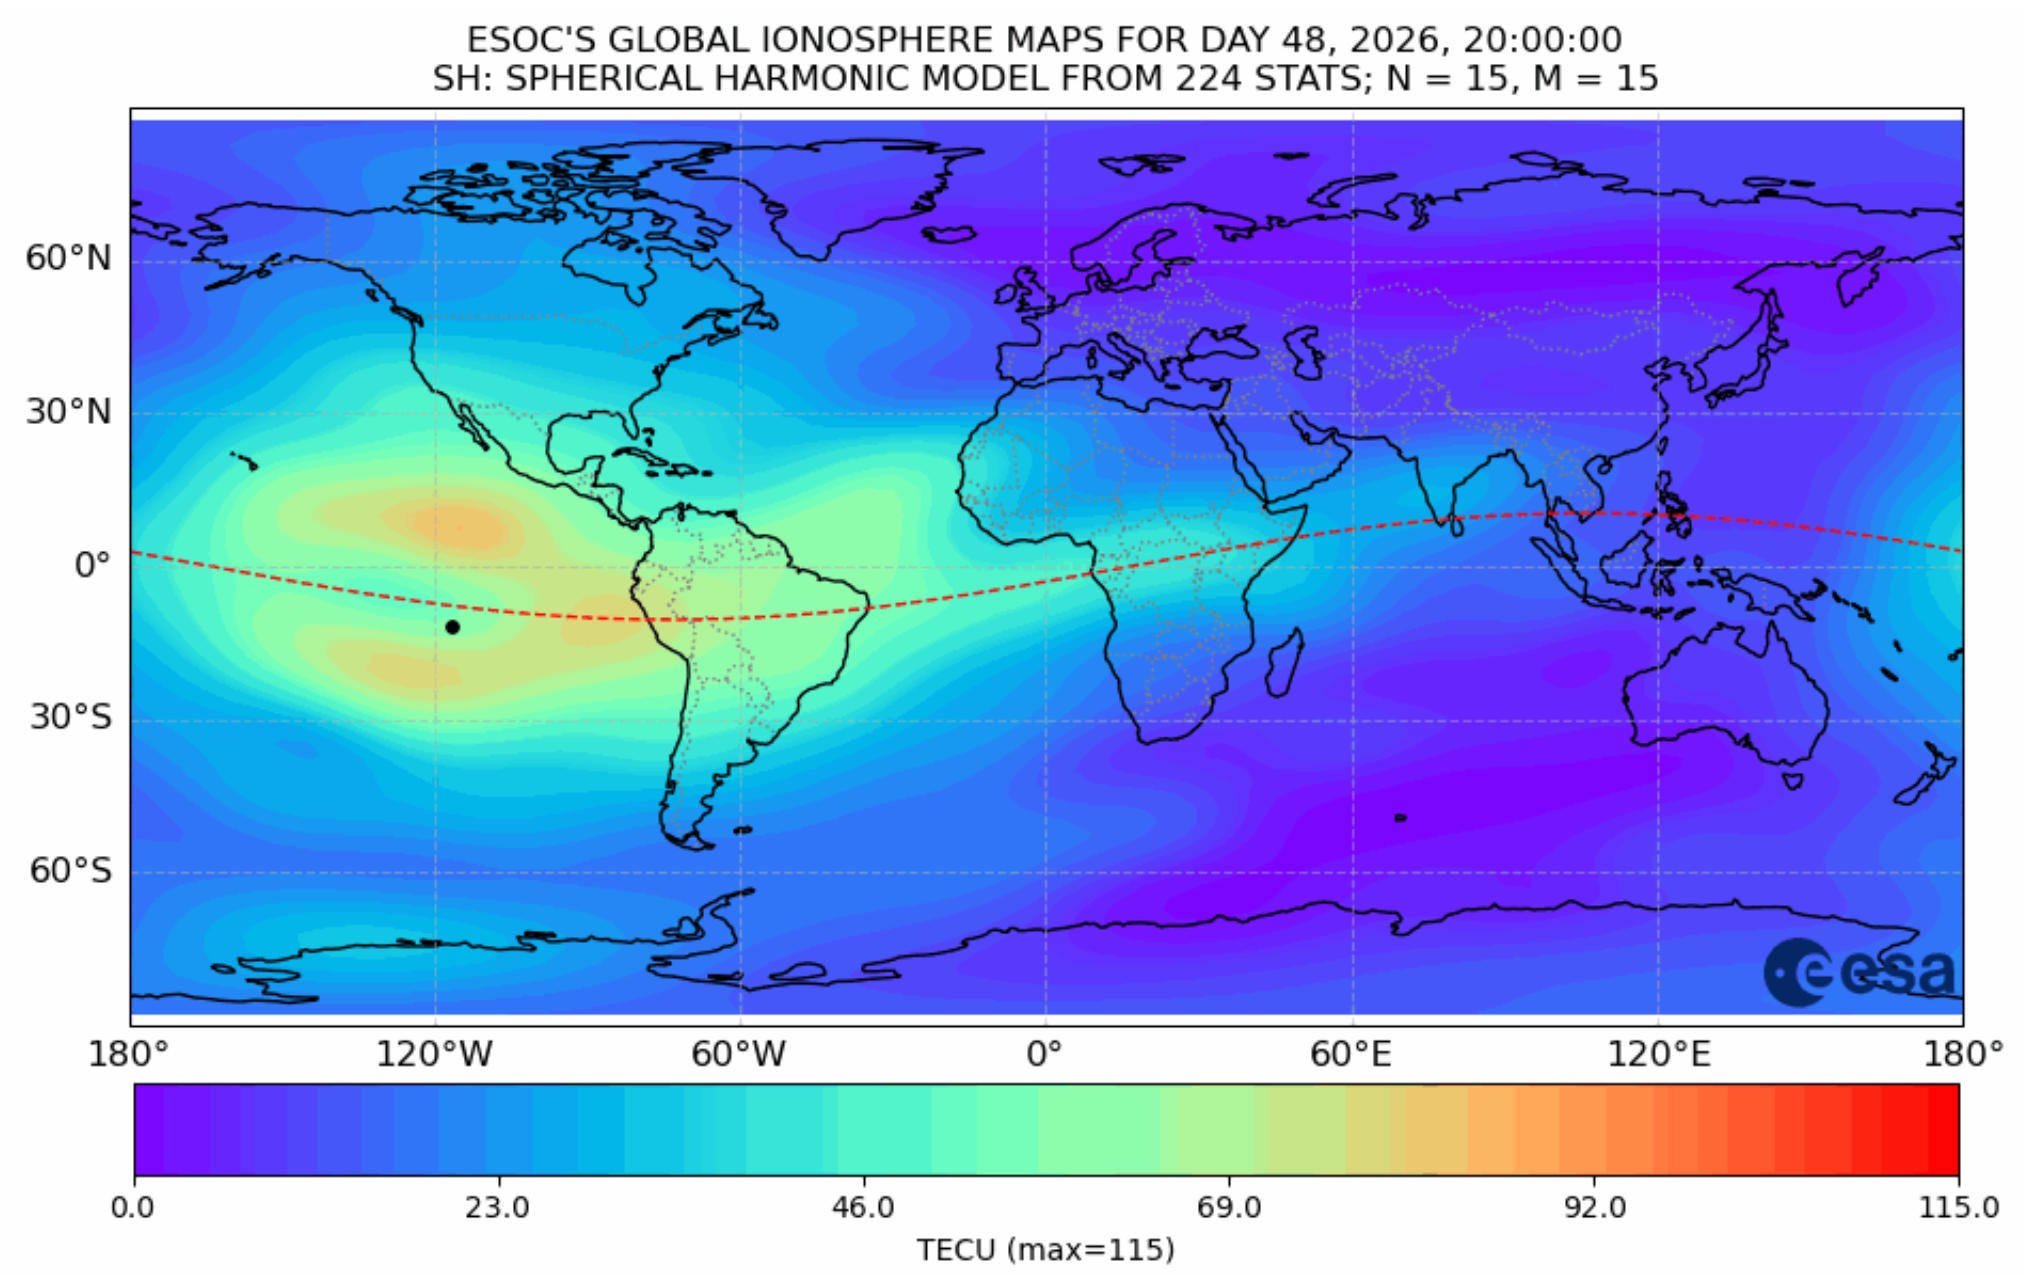
\includegraphics[width=0.47\linewidth]{figs/TECU_8pm.png} &
				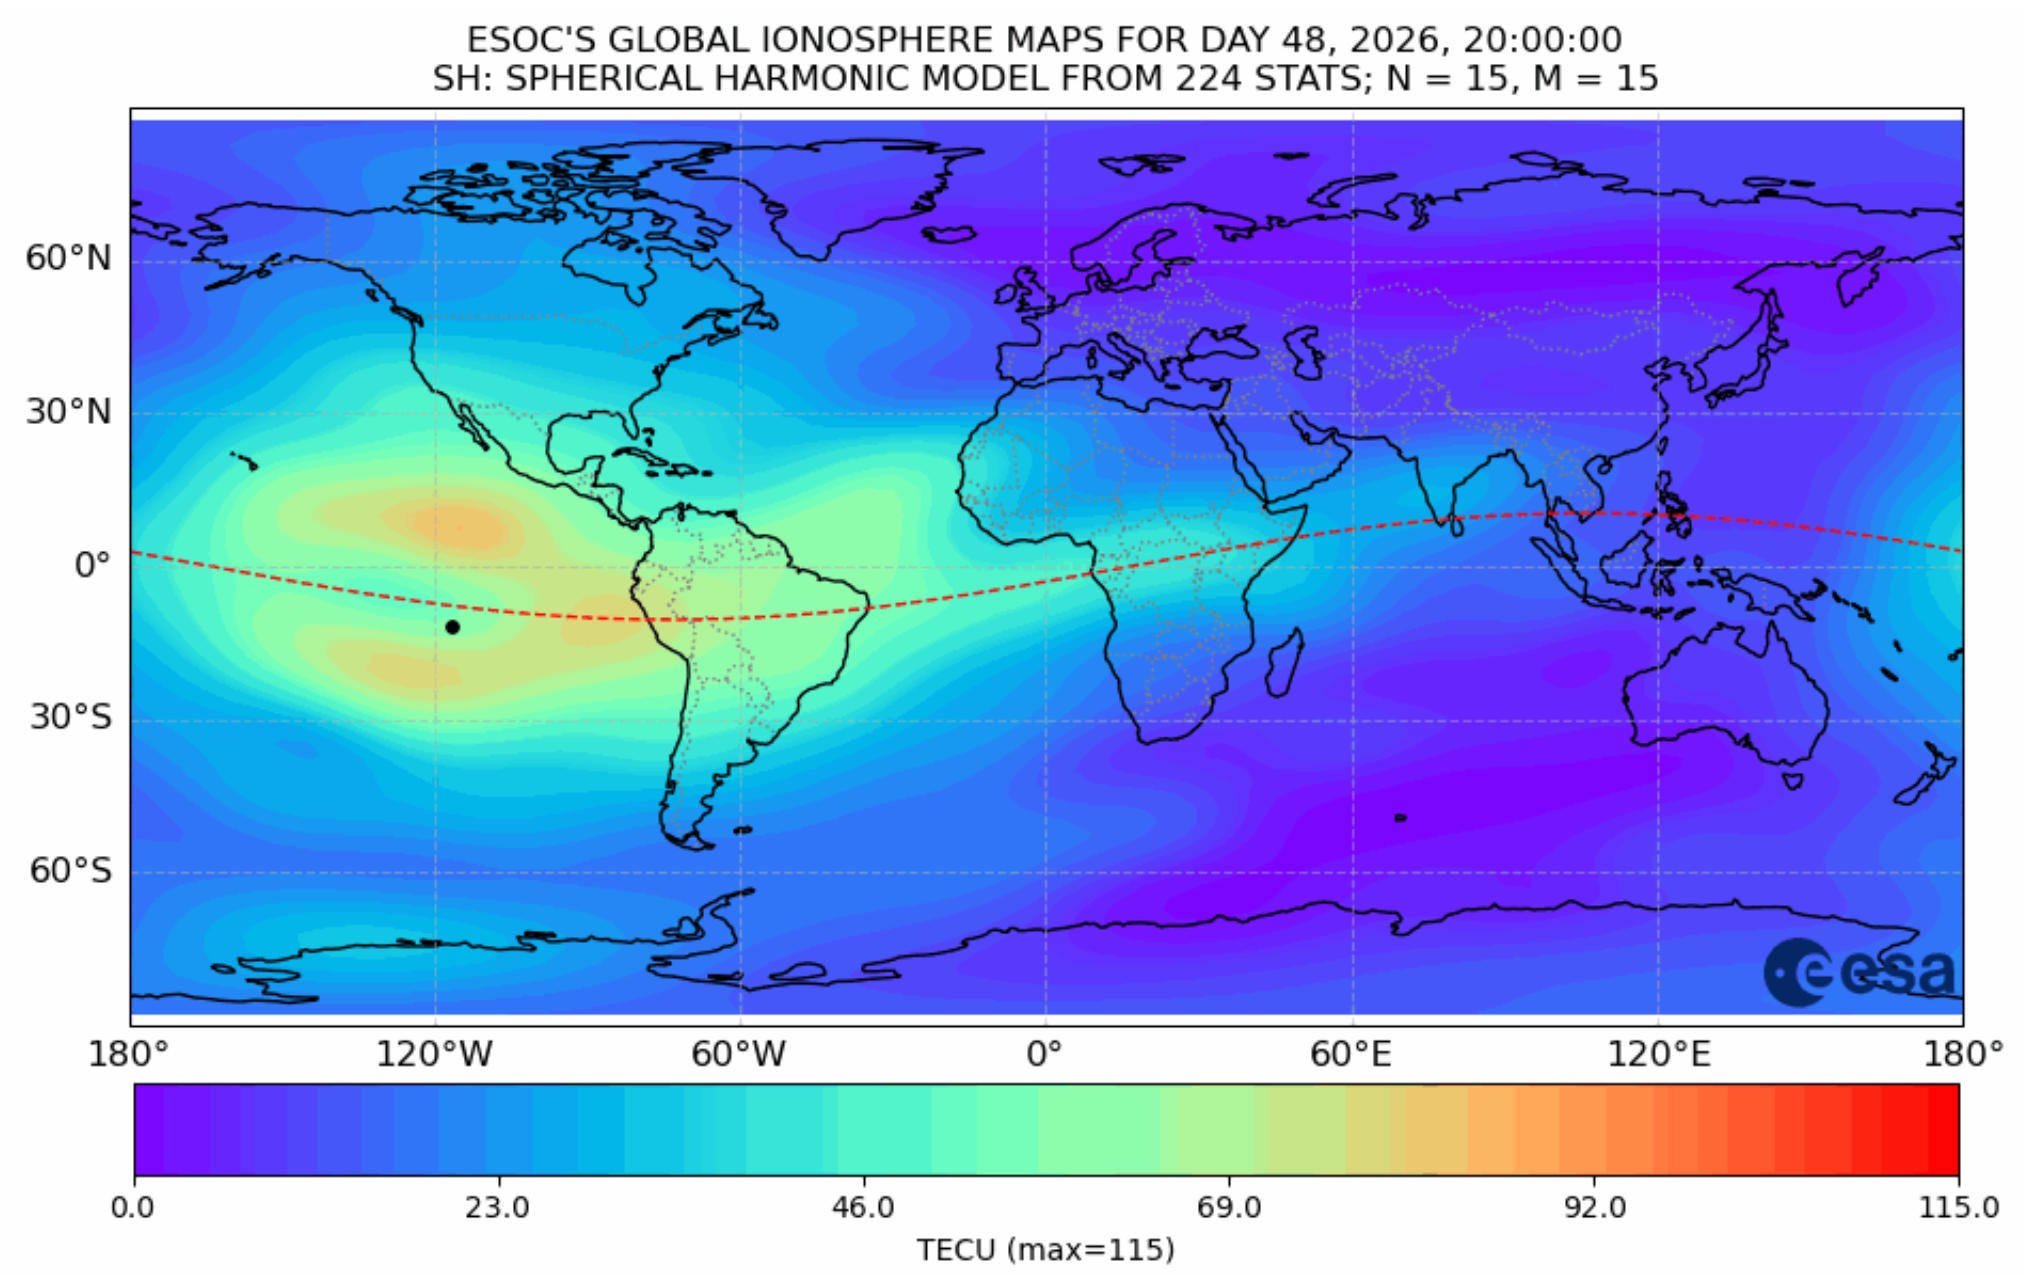
\includegraphics[width=0.47\linewidth]{figs/TECU_8pm.png}
			\end{tabular}
            \caption{Temporal evolution of the \cgls{tec} unit index.}
		\end{figure}
        \end{visibleenv}
	\end{columns}
\end{frame}


\section{Introduction}
\begin{frame}[<+->][t]{Introduction}
	Note: For each of the basic commands \textbackslash only, \textbackslash uncover, \textbackslash invisible and
\textbackslash alt there exists ``environment versions'': onlyenv, altenv, visibleenv, uncoverenv \& invisibleenv.
	\begin{align}
		\uncover<+->{A = & aL R^b \nonumber \\}
		\uncover<+->{R = & \left(\frac{A}{aL}\right)^{\frac{1}{b}}}
		\label{power_law}
	\end{align}
	\begin{visibleenv}<+->
		Applying the \(\ln\) transformation in both side of this equation, we have
		\begin{align}
			\uncover<+->{\ln R = & \frac{1}{b} \ln A - \frac{\ln \left(aL\right)}{b} \nonumber}
			\uncover<+->{\underbrace{\ln R}_{y} = & \underbrace{\frac{1}{b}}_{\theta_1} \underbrace{\ln A}_x \underbrace{- \frac{\ln \left(aL\right)}{b}}_{\theta_0} \nonumber}
		\end{align}
        
		\uncover<+->{Hence, we have a linear model, i.e., \(y = \theta_1 x + \theta_0\).}
	\end{visibleenv}
\end{frame}

\begin{frame}[<+->][t]
	\frametitle{teste}
	
	\only<2>{Only: Neither occupies space nor is visible}
	\visible<3>{Visible: Occupies space but is invisible}
	\uncover<4>{But uncover both occupies space and is visible} Final test
\end{frame}

\begin{frame}[t]
	\frametitle{Master Dissertation highlight's}
	Objetivo geral: Concepção da arquitetura digital do modem AFSK. Implementação do protótipo lógico no \textit{software} \textit{MATLAB/Simulink}. 

	\vspace{6pt}

	Objetivos específicos:
	\begin{itemize}
		\item Descrição matemática de uma nova arquitetura de modulador AFSK.
		\item Derivação do limite superior para a probabilidade de erro.
		\item Estimadores de fase e tempo para a nova arquitetura.
	\end{itemize}
\end{frame}

\begin{frame}
	\frametitle{teste}
	\begin{table}
		\begin{tabular}{|p{8cm} | l|}
			\hline
			Undergraduated in Electronic Engineering at Unifor(Universidade de Fortaleza) & 2013-2018 \\
			\hline
		\end{tabular}
	\end{table}
\end{frame}

\begin{frame}
	\frametitle{teste}

	\begin{columns}
		\column{0.5\textwidth}
		text text text text text text text text text text text text text text text text text text text text text text text text text text text text text text text text text text text text text text text text text text text text text text text text text text text text text text text text text text text text text text text text text text text text text text text text text text text text text text text text text text text text 
		\column{0.5\textwidth}
		text text text text text text text text text text text text text text text text text text text text text text text text text text text text text text text text text text text text text text text text text text text text text text text text text text text text text text text text text text text text text text text text text text text text text text text text text text text text text text text text text text text text 
	\end{columns}
\end{frame}

\begin{frame}[<+->][t]{Who am I?}
	Some personal information:
	\begin{itemize}
		\item Rubem Vasconcelos Pacelli, 27 years old.
		\item I am from Fortaleza, Ceará, Brazil.
	\end{itemize}
	\uncover<.->{Academic information:}
	\begin{itemize}
		\item \begin{tabular*}{0.9\textwidth}[t]{p{7cm}@{\extracolsep{\fill}}r}
			BSc in Electronic Engineering at \newline Unifor(Universidade de Fortaleza) & Jan 2013 -- Dec 2018 \end{tabular*}%\vspace{-7pt}
		\item \begin{tabular*}{0.9\textwidth}[t]{p{6.5cm}@{\extracolsep{\fill}}r}
			MSc in Teleinformatics Engineering at Federal University of Ceará.  & Jan 2019 -- \emph{Jun 2021} \end{tabular*}%\vspace{-7pt}
	\end{itemize}
\end{frame}


\begin{frame}[<+->]
	\frametitle{What is my technical skills?}

	\uncover{Programming (and hardware description) Languages:}
	\begin{itemize}
		\item Matlab/Simulink: 5 years of experience, approximately.
		\item Python: 2 years of intense usage.
		\item C, C++, VHDL, and Java: Secondary usage.
	\end{itemize}

	\uncover<+(1)->{Some further technical skills:}
	\begin{itemize}
		\item Git: Elementary concepts.
		\item \LaTeX: Elementary concepts.
	\end{itemize}

	\uncover<+(1)->{Language skills:}
	\begin{itemize}
		\item English: Full professional working proficiency (Level B2 on TOEFL IBT. Total score: 74 out of 120).
		\item Portuguese: Native Language.
	\end{itemize}

\end{frame}

\begin{frame}{Main challenges}
    \begin{itemize}
        \item The design of modern digital modems for the further development of CubeSat satellite systems;
        \item The usage of the software-defined radio (SDR) concept, combined with the  enhancement of digital signal processing techniques, FPGA (field-programmable gate array), and microelectronics, has motivated a new generation of TT\&C (telemetry, tracking and command) modules that \ul{brings hardware flexibility, but at the same time, matches with the current modulation schemes}.
    \end{itemize}
    \begin{textblock}{8}(1,4.5)
        The Viterbi algorithm is employed for the maximum likelihood sequence detection, and its statistics are feedbacked to estimate the phase and timing offset.
    \end{textblock}
\end{frame}

\end{document}